\section{Zasada działania układu i wyjaśnienie sygnałów}
Zaprojektowany układ jest asynchroniczny z prędkością transmisji $2400$Hz. Po rozpoczęciu transmisji nie można jej przerwać. Transmitowany jest ciąg 11 bitów w tym i każdy bit jest przesyłany co cykl zegarowy.\\
Na ciąg przesyłanych bitów (''zatrzasniete'') składa się:

\begin{itemize}
    \item jeden bit rozpoczęcia i jeden bit zakończenia transmisji
    \item osiem bitów treści (slowo-trans)
    \item jeden bit parzystości, sprawdzajacy czy transmisja była poprawna (w programie jest możliwość zmienienia bitu na ''Even'' lub ''Odd'')
\end{itemize}

Po zakończeniu transmisji zmienna ''transmisja'' spowrotem przyjmuje wartość $0$ i układ jest gotowy na przesłanie kolejnego ciągu znaków.

\begin{figure}[!htb]
    \centering
    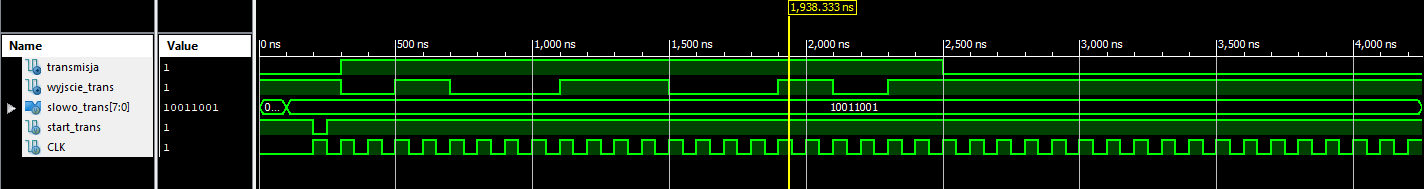
\includegraphics[width=18cm]{./Images/Symulacja.png}
    \caption*{Test układu przy pomocy symulacji}
\end{figure}

\section{Schemat blokowy}
Wstaw zdjęcie

\section{Kod VerilogMain}
\subsection{Całość kodu}
\begin{lstlisting}

`timescale 1ns / 1ps


module main(
    input CLK,
	 input CE,
	 input CD,
	 input SV,
	 output [3:0] out
    );


reg [3:0] current_value;
reg [3:0] next_value;

initial
begin
	current_value = 4'b0000;
end


always @(posedge CLK or negedge SV)
begin
	if ( SV == 0) 
	begin
		if ( CD == 0 ) current_value = 4'b0000;
		else current_value = 4'b1111;
	end
	else if ( CE == 1 )	current_value = next_value;
end


always @ (current_value or CD)
begin
	if (CD == 0)
	begin
		case(current_value)
			4'b0000 : next_value = 4'b0001; //0 kod Aikena
			4'b0001 : next_value = 4'b0010; //1 
			4'b0010 : next_value = 4'b0011; //2
			4'b0011 : next_value = 4'b0100; //3
			4'b0100 : next_value = 4'b1011; //4
			4'b1011 : next_value = 4'b1100; //5
			4'b1100 : next_value = 4'b1101; //6
			4'b1101 : next_value = 4'b1110; //7
			4'b1110 : next_value = 4'b1111; //8
			4'b1111 : next_value = 4'b0000; //9
		endcase
	end
	else
	begin
		case(current_value)
			4'b0000 : next_value = 4'b1111; //0 kod Aikena
			4'b0001 : next_value = 4'b0000; //1 
			4'b0010 : next_value = 4'b0001; //2
			4'b0011 : next_value = 4'b0010; //3
			4'b0100 : next_value = 4'b0011; //4
			4'b1011 : next_value = 4'b0100; //5
			4'b1100 : next_value = 4'b1011; //6
			4'b1101 : next_value = 4'b1100; //7
			4'b1110 : next_value = 4'b1101; //8
			4'b1111 : next_value = 4'b1110; //9
		endcase
	end
end




assign out = current_value;

endmodule

\end{lstlisting}

\subsection{Wyjasnienie poszczególnych elementów kodu}
Pierwszym elementem jest dzielnik sygnału zegarowego. Zmiana w ''CLK2380'' następuje co 42 cykle sygnału zegarowego, dzięki czemu wewnętrzny sygnał zegarowy wynosi dokładnie 2380 Hz.
\begin{lstlisting}
    library IEEE;
    use IEEE.STD_LOGIC_1164.ALL;
    use IEEE.STD_LOGIC_ARITH.ALL;
    use IEEE.STD_LOGIC_UNSIGNED.ALL;
    
    entity licznik is
        Port ( zegar : in STD_LOGIC;
                  reset : in STD_LOGIC;
               stop : in STD_LOGIC;
                  wyjscie1 : out STD_LOGIC_VECTOR (3 downto 0);
                  wyjscie2 : out STD_LOGIC_VECTOR (3 downto 0);
                  wyjscie3 : out STD_LOGIC_VECTOR (3 downto 0);
                  wyjscie4 : out STD_LOGIC_VECTOR (3 downto 0));
    end licznik;
    
    architecture Behavioral of licznik is
    
    signal liczba1 : STD_LOGIC_VECTOR (3 downto 0) := "0000";
    signal liczba2 : STD_LOGIC_VECTOR (3 downto 0) := "0000";
    signal liczba3 : STD_LOGIC_VECTOR (3 downto 0) := "0000";
    signal liczba4 : STD_LOGIC_VECTOR (3 downto 0) := "0000";
     
    begin
     
    process(zegar, reset)
    begin
        if reset = '0' then
            liczba1 <= "0000";
            liczba2 <= "0000";
            liczba3 <= "0000";
            liczba4 <= "0000";
            
        elsif zegar = '1' and zegar'event then
                if stop = '1' then			
                    if liczba1 = "1001" then
                        liczba1 <= "0000";
                        
                        if liczba2 = "1001" then
                            liczba2 <= "0000";
                            
                            if liczba3 = "1001" then
                                liczba3 <= "0000";
                                
                                if liczba4 = "1001" then
                                    liczba4 <= "0000";
                                else
                                    liczba4 <= liczba4 + 1;
                                end if;
                                
                            else
                                liczba3 <= liczba3 + 1;
                            end if;		
                            
                        else
                            liczba2 <= liczba2 + 1;
                        end if;
                        
                    else
                        liczba1 <= liczba1 + 1;
                    end if;
                end if;
        end if;
    end process;
    
    wyjscie1 <= liczba1;
    wyjscie2 <= liczba2;
    wyjscie3 <= liczba3;
    wyjscie4 <= liczba4;
    
    end Behavioral;
\end{lstlisting}

Drugim elementem jest przypisanie odpowiednich bitów do później transmitowanej sekwencji (z możliwością wyboru czy posługujemy się bitem parzystości ''Odd'', czy ''Even'')
\begin{lstlisting}
	always @(slowo_trans or start_trans)
	begin
		if(start_trans == 0)
		begin
			zatrzasniete[0] <= 0;
			zatrzasniete[8:1] <= slowo_trans[7:0];
			
			if (jaki_parz == 0)
				zatrzasniete[9] <= (^slowo_trans[7:0]);
			else
				zatrzasniete[9] <= (~^slowo_trans[7:0]);
			
			zatrzasniete[10] <= 1;
		end
	end
\end{lstlisting}

kolejnym elementem jest przesyłanie bit po bicie transmisji, po zmianie stanu. Stan jest zależny od CLK2380. Możliwe jest równierz określenie czy zostanie przesłany bit parzystości czy nie.
\begin{lstlisting}
	always @(posedge CLK2380 or negedge start_trans)
	begin
		if(start_trans == 0)
			stan <= 0;
		else if (stan == 4'b1001 && czy_parz == 0)
			stan <= stan + 2;
		else if (stan < 12)
			stan <= stan + 1;
	end
	
	always @(stan or zatrzasniete)
	begin
		case (stan)
			4'b0000 : wyjscie = 1;
			4'b0001 : wyjscie = zatrzasniete[0];
			4'b0010 : wyjscie = zatrzasniete[1];
			4'b0011 : wyjscie = zatrzasniete[2];
			4'b0100 : wyjscie = zatrzasniete[3];
			4'b0101 : wyjscie = zatrzasniete[4];
			4'b0110 : wyjscie = zatrzasniete[5];
			4'b0111 : wyjscie = zatrzasniete[6];
			4'b1000 : wyjscie = zatrzasniete[7];
			4'b1001 : wyjscie = zatrzasniete[8];
			4'b1010 : wyjscie = zatrzasniete[9];
			default : wyjscie = zatrzasniete[10];
		endcase
	end
\end{lstlisting}

\section{Test układu}
\subsection{symulacja w programie}
\begin{lstlisting}
    `timescale 1ns / 1ps

    module symulacja;
        // Inputs
        reg [7:0] slowo_trans;
        reg start_trans;
        reg CLK;
    
        // Outputs
        wire transmisja;
        wire wyjscie_trans;
    
        // Instantiate the Unit Under Test (UUT)
        main uut (
            .slowo_trans(slowo_trans), 
            .start_trans(start_trans), 
            .CLK(CLK), 
            .transmisja(transmisja), 
            .wyjscie_trans(wyjscie_trans)
        );
    
        initial begin
            // Initialize Inputs
            slowo_trans = 0;
            start_trans = 1;
            CLK = 0;
    
            // Wait 100 ns for global reset to finish
            #100;
           
            slowo_trans = 8'b10011001;
             
            #100;
            
            start_trans = 0;
            CLK = 1;
            
            #50;
            start_trans = 1;
            CLK = 0;
            
            #50
            CLK = 1;
            #50
            CLK = 0;
            #50
            CLK = 1;
            #50
            CLK = 0;
            #50
            CLK = 1;
            
            ...

            #50
            CLK = 0;
        end
    endmodule        
\end{lstlisting}
\begin{figure}[!htb]
    \centering
    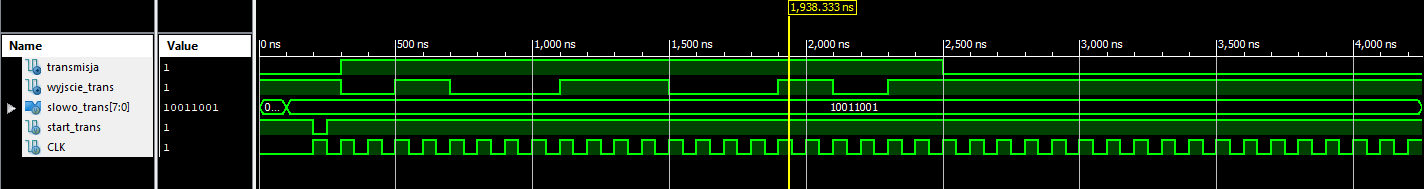
\includegraphics[width=18cm]{./Images/Symulacja.png}
    \caption*{Test układu przy pomocy symulacji}
\end{figure}
\clearpage

\subsection{Zdjęcia z testu na oscyloskopie}
\begin{figure}[!htb]
    \centering
    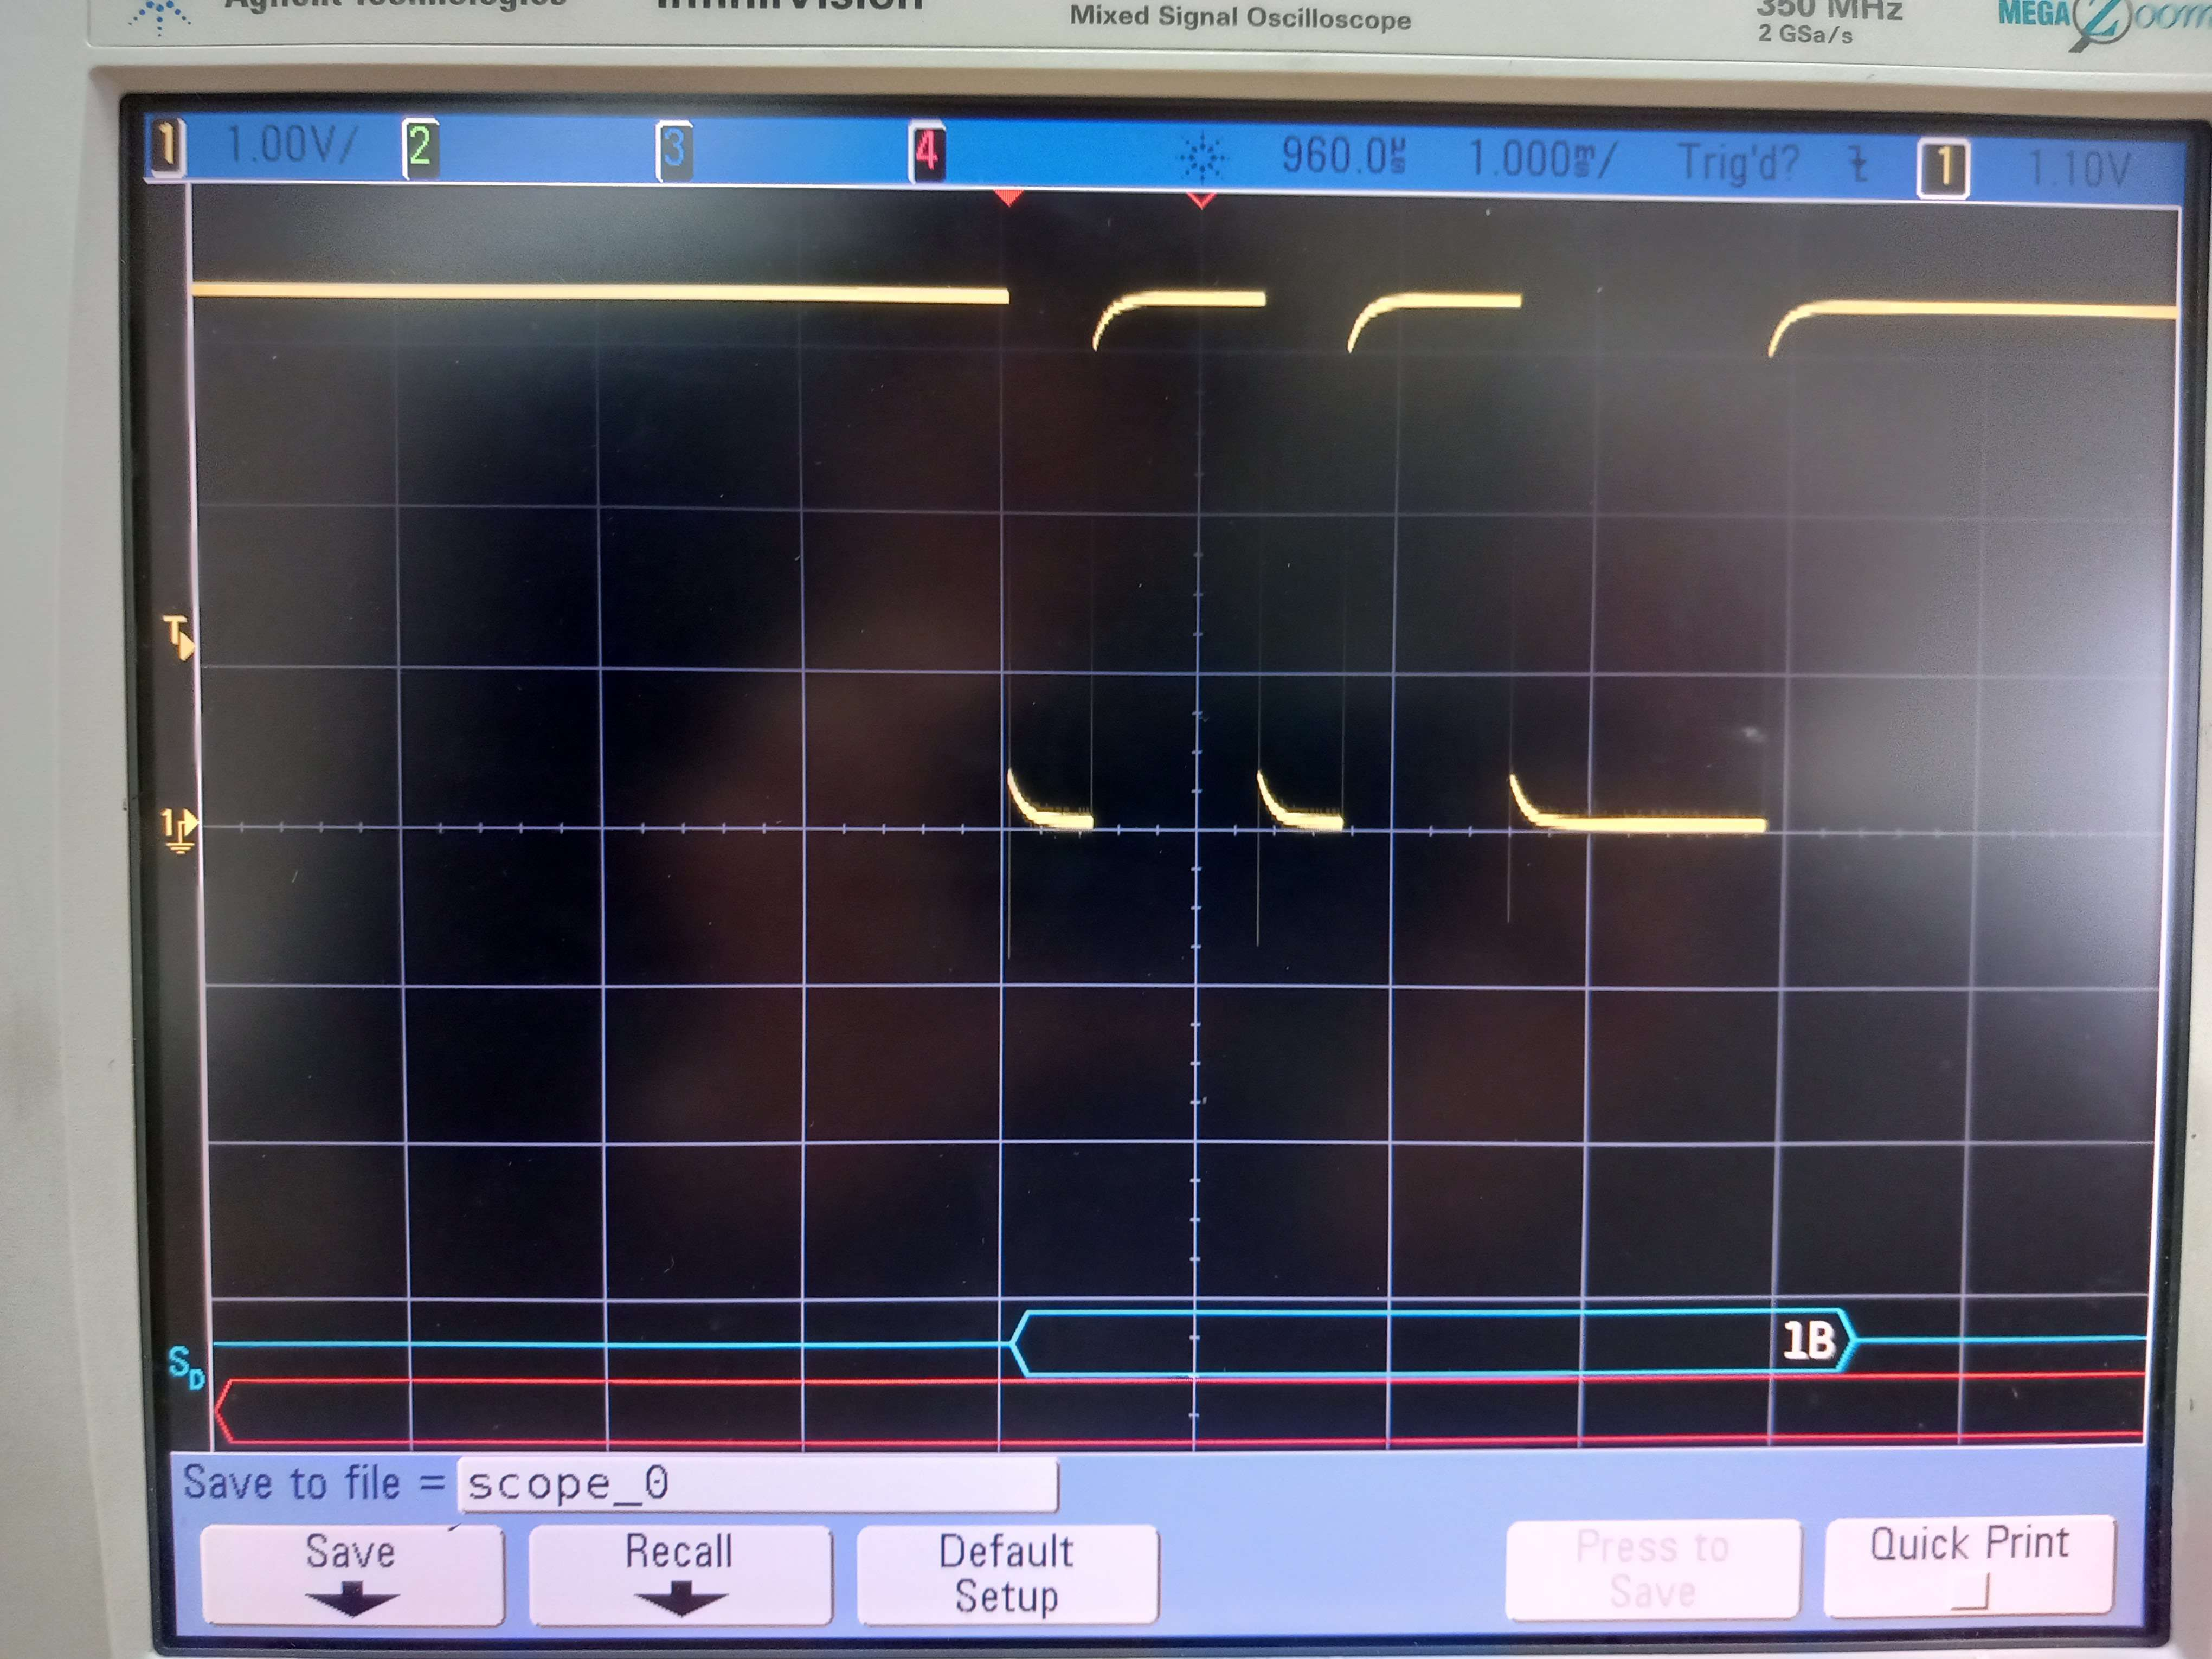
\includegraphics[width=18cm]{./Images/oscy.jpg}
    \caption*{Test układu przy pomocy oscyloskopu}
\end{figure}